%\section{声速与马赫数}
\subsection{微弱扰动的一维传播}
\begin{frame}{微弱扰动的一维传播过程}
  \begin{figure}
    \begin{tikzpicture}
      \begin{scope}
      \draw[thick] (0,0) -- (4,0);
      \draw[thick] (0,1.5) -- (4,1.5);
      \foreach \p in 
    {0.1, 0.2, 0.3, 0.4, 0.5, 0.6, 0.7, 0.8, 0.9, 1.0,
     1.1, 1.2, 1.3, 1.4, 1.5, 1.6, 1.7, 1.8, 1.9, 2.0,
     2.1, 2.2, 2.3, 2.4, 2.5, 2.6, 2.7, 2.8, 2.9, 3.0,
     3.1, 3.2, 3.3, 3.4, 3.5, 3.6, 3.7, 3.8, 3.9}
     {
      \draw[thin] (\p, 0) -- ++(-45:0.1);
      \draw[thin] (\p, 1.5) -- ++(45:0.1);
     }
     \draw[dashed,thin] (2,0) node[below]{$n$} -- (2,1.5) node[above]{$m$};
     \draw[-latex,thick] (2,0.75) -- node[midway,above]{$c$} ++(1,0);
     \node at (3.5, 1.2) {$p_{1}$};
     \node at (3.5, 0.8) {$\rho_{1}$};
     \node at (3.5, 0.4) {$T_{1}$};
     \node at (1.5, 1.2) {$p_{2}$};
     \node at (1.5, 0.8) {$\rho_{2}$};
     \node at (1.5, 0.4) {$T_{2}$};

     \draw[thin] (0.8,0) -- (0.8,1.5);
     \draw[thin] (1.0,0) -- (1.0,1.5);
     \draw[thick,fill=black] (0.6,0.6) -- (0.8, 0.6) -- (0.8, 0.9) -- (0.6,0.9) -- cycle;
     \draw[-latex,thick] (0.1,0.75) -- node[midway,above]{$\mathrm{d}v$}(0.6,0.75);
   \end{scope}

     \begin{scope}[yshift=-2.5cm]
       \draw[-latex, thin] (0,0) -- (4,0) node[below]{$x$};
       \draw[-latex, thin] (0,0) -- (0,2) node[left]{$p$};
       \draw[thick] (0,1.5) -- node[midway,above]{$p_{2}$} (2,1.5);
       \draw[thick] (2,1) -- node[midway,above]{$p_{1}$} (4,1);
       \draw[thin,dashed] (2,0) -- (2,2);
     \end{scope}

     \begin{scope}[yshift=-4cm]
       \draw[-latex, thin] (0,0) -- (4,0) node[below]{$x$};
       \draw[-latex, thin] (0,-0.6) -- (0,1) node[left]{$v$};
       \draw[thick] (0,0.5) -- node[midway,above]{$\mathrm{d}v$} (2,.5);
       \draw[thin,dashed] (2,-0.6) -- (2,1);
       \node at (2,-0.6) [anchor=north]{(a)活塞向右移动,压缩波};
     \end{scope}


     \begin{scope}[xshift=6cm]
      \draw[thick] (0,0) -- (4,0);
      \draw[thick] (0,1.5) -- (4,1.5);
      \foreach \p in 
    {0.1, 0.2, 0.3, 0.4, 0.5, 0.6, 0.7, 0.8, 0.9, 1.0,
     1.1, 1.2, 1.3, 1.4, 1.5, 1.6, 1.7, 1.8, 1.9, 2.0,
     2.1, 2.2, 2.3, 2.4, 2.5, 2.6, 2.7, 2.8, 2.9, 3.0,
     3.1, 3.2, 3.3, 3.4, 3.5, 3.6, 3.7, 3.8, 3.9}
     {
      \draw[thin] (\p, 0) -- ++(-45:0.1);
      \draw[thin] (\p, 1.5) -- ++(45:0.1);
     }
     \draw[dashed,thin] (2,0) node[below]{$n$} -- (2,1.5) node[above]{$m$};
     \draw[-latex,thick] (2,0.75) -- node[midway,above]{$c$} ++(1,0);
     \node at (3.5, 1.2) {$p_{1}$};
     \node at (3.5, 0.8) {$\rho_{1}$};
     \node at (3.5, 0.4) {$T_{1}$};
     \node at (1.5, 1.2) {$p_{2}$};
     \node at (1.5, 0.8) {$\rho_{2}$};
     \node at (1.5, 0.4) {$T_{2}$};

     \draw[thin] (0.8,0) -- (0.8,1.5);
     \draw[thin] (1.0,0) -- (1.0,1.5);
     \draw[thick,fill=black] (0.6,0.6) -- (0.8, 0.6) -- (0.8, 0.9) -- (0.6,0.9) -- cycle;
     \draw[-latex,thick] (0.6,0.75) -- node[midway,above]{$\mathrm{d}v$}(0.1,0.75);
   \end{scope}

     \begin{scope}[xshift=6cm,yshift=-2.5cm]
       \draw[-latex, thin] (0,0) -- (4,0) node[below]{$x$};
       \draw[-latex, thin] (0,0) -- (0,2) node[left]{$p$};
       \draw[thick] (0,1) -- node[midway,above]{$p_{2}$} (2,1);
       \draw[thick] (2,1.5) -- node[midway,above]{$p_{1}$} (4,1.5);
       \draw[thin,dashed] (2,0) -- (2,2);
     \end{scope}

     \begin{scope}[xshift=6cm,yshift=-4cm]
       \draw[-latex, thin] (0,0) -- (4,0) node[below]{$x$};
       \draw[-latex, thin] (0,-0.6) -- (0,1) node[left]{$v$};
       \draw[thick] (0,-0.5) -- node[midway,above]{$\mathrm{d}v$} (2,-0.5);
       \draw[thin,dashed] (2,-0.6) -- (2,1);
       \node at (2,-0.6) [anchor=north]{(b)活塞向左移动,膨胀波};
     \end{scope}
    \end{tikzpicture}
  \end{figure}
\end{frame}

\subsection{声速}
\begin{frame}{声速}
  \begin{itemize}
    \item 微弱扰动波在流体介质中的传播速度$c$称为声速
  \end{itemize}
  \begin{figure}
  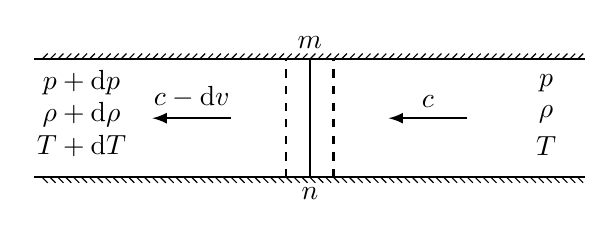
\begin{tikzpicture}
    \draw[thick] (0,0) -- (7,0);
    \draw[thick] (0,1.5) -- (7,1.5);
    \draw[thick] (3.5,0) node[anchor=north]{$n$} -- (3.5,1.5) node[anchor=south]{$m$};
    \draw[thick,dashed] (3.2,0) -- (3.2,1.5);
    \draw[thick,dashed] (3.8,0) -- (3.8,1.5);
    \draw[thick,-latex] (2.5,0.75) -- node[midway,above]{$c-\mathrm{d}v$} (1.5,0.75);
    \draw[thick,-latex] (5.5,0.75) -- node[midway,above]{$c$} (4.5,0.75);
    \node at (6.5, 1.2) {$p$};
    \node at (6.5, 0.8) {$\rho$};
    \node at (6.5, 0.4) {$T$};
    \node at (0.6, 1.2) {$p+\mathrm{d}p$};
    \node at (0.6, 0.8) {$\rho+\mathrm{d}\rho$};
    \node at (0.6, 0.4) {$T+\mathrm{d}T$};
    \foreach \p in 
    {0.1, 0.2, 0.3, 0.4, 0.5, 0.6, 0.7, 0.8, 0.9, 1.0,
     1.1, 1.2, 1.3, 1.4, 1.5, 1.6, 1.7, 1.8, 1.9, 2.0,
     2.1, 2.2, 2.3, 2.4, 2.5, 2.6, 2.7, 2.8, 2.9, 3.0,
     3.1, 3.2, 3.3, 3.4, 3.5, 3.6, 3.7, 3.8, 3.9, 4.0,
     4.1, 4.2, 4.3, 4.4, 4.5, 4.6, 4.7, 4.8, 4.9, 5.0,
     5.1, 5.2, 5.3, 5.4, 5.5, 5.6, 5.7, 5.8, 5.9, 6.0,
     6.1, 6.2, 6.3, 6.4, 6.5, 6.6, 6.7, 6.8, 6.9}
    {
      \draw[thin] (\p, 0) -- ++(-45:0.1);
      \draw[thin] (\p, 1.5) -- ++(45:0.1);
    }
  \end{tikzpicture}
  \end{figure}
  \vspace*{-0.5em}
  连续性方程:
  \vspace*{-1.3em}
  \begin{equation*}
  c\rho A\mathrm{d}t
  =
  (c-\mathrm{d}v)(\rho+\mathrm{d}\rho)A\mathrm{d}t
  \end{equation*}
  \begin{equation*}
  c\mathrm{d}\rho
  =
  \rho\mathrm{d}v
  \end{equation*}

  \vspace*{0.5em}
  动量方程:
  \vspace*{-1.8em}
  \begin{equation*}
  c\rho A\mathrm{d}t
  \frac{[(c-\mathrm{d}v)-c]}{\mathrm{d}t}
  =
  [p-(p+\mathrm{d}p)]A
  \end{equation*}
  \begin{equation*}
  c\rho\mathrm{d}v
  =
  \mathrm{d}p
  \end{equation*}
  \begin{equation*}
  c =
  \sqrt{\frac{\mathrm{d}p}{\mathrm{d}\rho}}
  \end{equation*}
\end{frame}

\begin{frame}{声速——续}
 气体为完全气体:
 \begin{equation*}
   \frac{p}{\rho^{\gamma}}
   =
   \mathrm{C}
 \end{equation*}
 \begin{equation*}
 \frac{\mathrm{d} p}{\mathrm{d} \rho}
 =
 \gamma \frac{p}{\rho}
 =
 \gamma RT
 \end{equation*}
 \begin{equation*}
 c
 =
 \sqrt{\frac{\mathrm{d}p}{\mathrm{d}\rho}}
 =
 \sqrt{\gamma\frac{p}{\rho}}
 =
 \sqrt{\gamma RT}
 \end{equation*}
 对于空气
% ($20^{\circ}\!\mathrm{C}$)
 ,$R=287\mathrm{J/kg\cdot K}$,$\gamma=1.4$
 \begin{equation*}
   c = 20.05\sqrt{T}
 \end{equation*}
 当$T=288.2\mathrm{K}=15^{\circ}\!\mathrm{C}$,$c=340.3\mathrm{m/s}$
\end{frame}

\begin{frame}{声速讨论}
  \vspace*{-1em}
  \begin{equation*}
    c = \sqrt{\gamma\frac{p}{\rho}} = \sqrt{\gamma RT}
  \end{equation*}
  \onslide<2->{
  \vspace*{-1em}
    \begin{block}{讨论}
  \begin{itemize}
    \item<2-|alert@2> 气体声速随气体的状态参数变化$c=f(p,\rho,R,T)$
    \item<3-|alert@3> 在同一流体介质中,各个点的瞬时状态参数是不同的,因而各个点的声速是不同的
    \item<4-|alert@4> 对非定常流,声速是空间和时间的函数,即$c=f(x,y,z,t)$
    \item<5-|alert@5> 对定常流,声速是空间的函数,即$c=f(x,y,z)$
    \item<6-|alert@6> 一般情况下,所提到的声速是指当地声速
    \item<7-|alert@7> 气体声速可作为判别气体压缩性标准,
      $
      \displaystyle
        E_{v}
        =
        \frac{\mathrm{d}p}{\mathrm{d}\rho/\rho}
        =
        \rho c^2
        $
        \begin{itemize}
          \item 流体可压缩性大的,$E_{v}$小,声速低
          \item 流体可压缩性小的,$E_{v}$大,声速高
        \end{itemize}
  \end{itemize}
\end{block}
}
\end{frame}

\subsection{气体流动分类}
\begin{frame}{气体流动分类、马赫数}
 \begin{block}{气体流动分类}
   \begin{enumerate}
     \item 当流速低于声速时,为亚声速流动
     \item 当流速等于声速时,为声速流动
     \item 当流速高于声速时,为超声速流动
   \end{enumerate}
 \end{block} 
 通常用无量纲数$\mathrm{Ma}$作为流动类型判别标准
 \begin{equation*}
   \mathrm{Ma}
   =
   \frac{v}{c}
 \end{equation*}
 \vspace*{-1.5em}
 \begin{block}{气体流动分类判别}
   \begin{enumerate}
     \item $v<c$或$\mathrm{Ma}<1$,为亚声速流动
     \item $v=c$或$\mathrm{Ma}=1$,为声速流动
     \item $v>c$或$\mathrm{Ma}>1$,为超声速流动
   \end{enumerate}
 \end{block} 
\end{frame}

\begin{frame}{马赫数讨论}
  \begin{equation*}
    \mathrm{Ma}
    =
    \frac{v}{c}
  \end{equation*}
  对于完全气体
  \begin{equation*}
    \mathrm{Ma}^{2}
    =
    \frac{v^{2}}{c^{2}}
    =
    \frac{v^{2}}{\gamma RT}
  \end{equation*}
  \onslide<2->{
  \begin{block}{讨论}
    \begin{itemize}
      \item<2-|alert@2> $v^{2}$表示气体宏观运动的动能大小
      \item<3-|alert@3> $T$表示气体的内能大小
      \item<4-|alert@4> $\mathrm{Ma}$表示气体宏观运动的动能与气体内能之比
      \item<5-|alert@5> $\mathrm{Ma}$小,则气体内能大而宏观动能小
      \item<6-|alert@6> $\mathrm{Ma}$大,则气体宏观动能大而内能小
    \end{itemize}
  \end{block}
}
\end{frame}

\begin{frame}{举例}
  \begin{block}{例:有一喷气式发动机,其尾部喷管出口处,气流的速度为
    $v=556\mathrm{m/s}$,气流的温度为$T=860\mathrm{K}$,气流的绝热指数
  $\gamma=1.33$,气体常数$R=287\mathrm{J/(kg\cdot K)}$,试求喷管出口处气流的声速
和马赫数,并确定流动类型。}
解:
   \begin{equation*}
   c
   =
   \sqrt{\gamma RT}
   =
   \sqrt{1.33\times 287 \times 860}
   =
   573\mathrm{m/s}
   \end{equation*} 
   \begin{equation*}
     \mathrm{Ma}
     =
     \frac{v}{c}
     =
     \frac{556}{573}
     =
     0.97 
   \end{equation*}
   $\mathrm{Ma}=0.97<1$,亚声速流动。
  \end{block}
\end{frame}
